\documentclass[tikz,border=8pt]{standalone}
\usepackage{amsmath}
\usepackage{pgfplots}
\pgfplotsset{compat=1.18}
\begin{document}
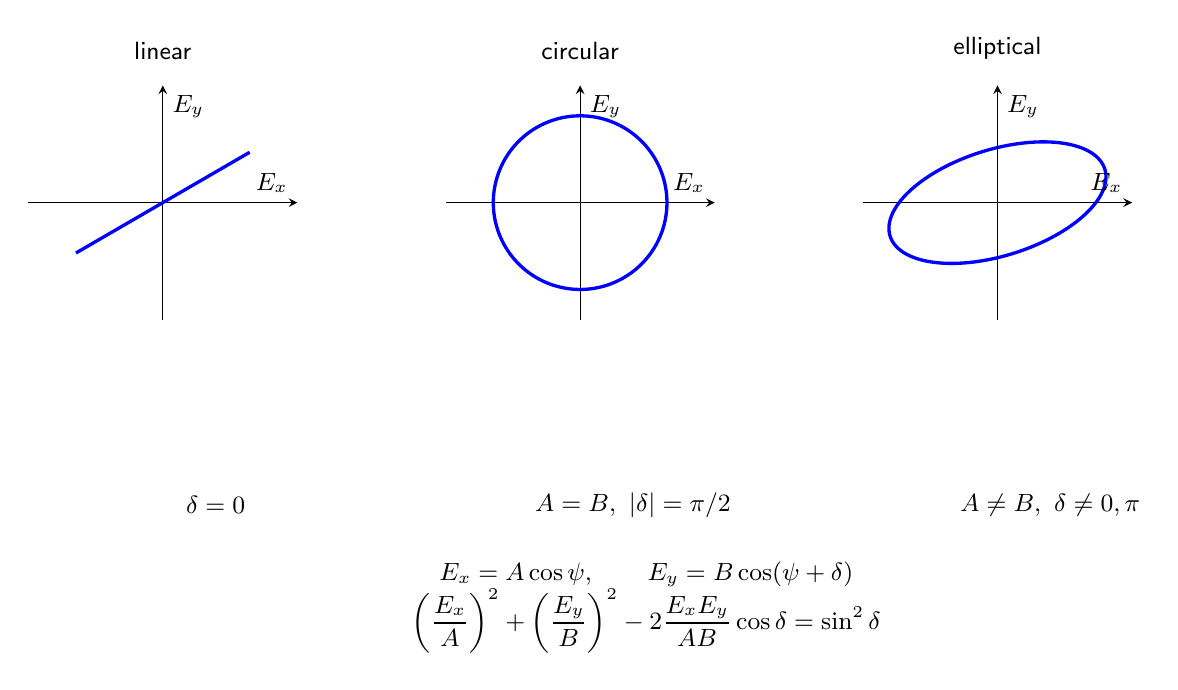
\begin{tikzpicture}[font=\sffamily\small]
    \begin{scope}
    \begin{axis}[
      width=5cm,height=5cm,axis equal image,
      axis lines=middle,xmin=-1.55,xmax=1.55,ymin=-1.35,ymax=1.35,
      xlabel={$E_x$},ylabel={$E_y$},xtick=\empty,ytick=\empty,
      title={linear}]
      \addplot[blue,very thick,domain=0:360,samples=180,variable=\x]
        ({cos(\x)},{.58*cos(\x)});
    \end{axis}
    \end{scope}
    \begin{scope}[xshift=5.3cm]
    \begin{axis}[
      width=5cm,height=5cm,axis equal image,
      axis lines=middle,xmin=-1.55,xmax=1.55,ymin=-1.35,ymax=1.35,
      xlabel={$E_x$},ylabel={$E_y$},xtick=\empty,ytick=\empty,
      title={circular}]
      \addplot[blue,very thick,domain=0:360,samples=180,variable=\x]
        ({cos(\x)},{sin(\x)});
    \end{axis}
    \end{scope}
    \begin{scope}[xshift=10.6cm]
    \begin{axis}[
      width=5cm,height=5cm,axis equal image,
      axis lines=middle,xmin=-1.55,xmax=1.55,ymin=-1.35,ymax=1.35,
      xlabel={$E_x$},ylabel={$E_y$},xtick=\empty,ytick=\empty,
      title={elliptical}]
      \addplot[blue,very thick,domain=0:360,samples=180,variable=\x]
        ({1.25*cos(\x)},{.7*cos(\x+65)});
    \end{axis}
    \end{scope}
  \node at (2.38,-2.35) {$\delta=0$};
  \node at (7.68,-2.35) {$A=B,\ |\delta|=\pi/2$};
  \node at (12.98,-2.35) {$A\ne B,\ \delta\ne0,\pi$};
  \node[align=center] at (7.85,-3.65)
    {$\displaystyle E_x=A\cos\psi,\qquad E_y=B\cos(\psi+\delta)$\\
     $\displaystyle \left(\frac{E_x}{A}\right)^2+\left(\frac{E_y}{B}\right)^2
       -2\frac{E_xE_y}{AB}\cos\delta=\sin^2\delta$};
\end{tikzpicture}
\end{document}
